\begin{figure*}[h]
    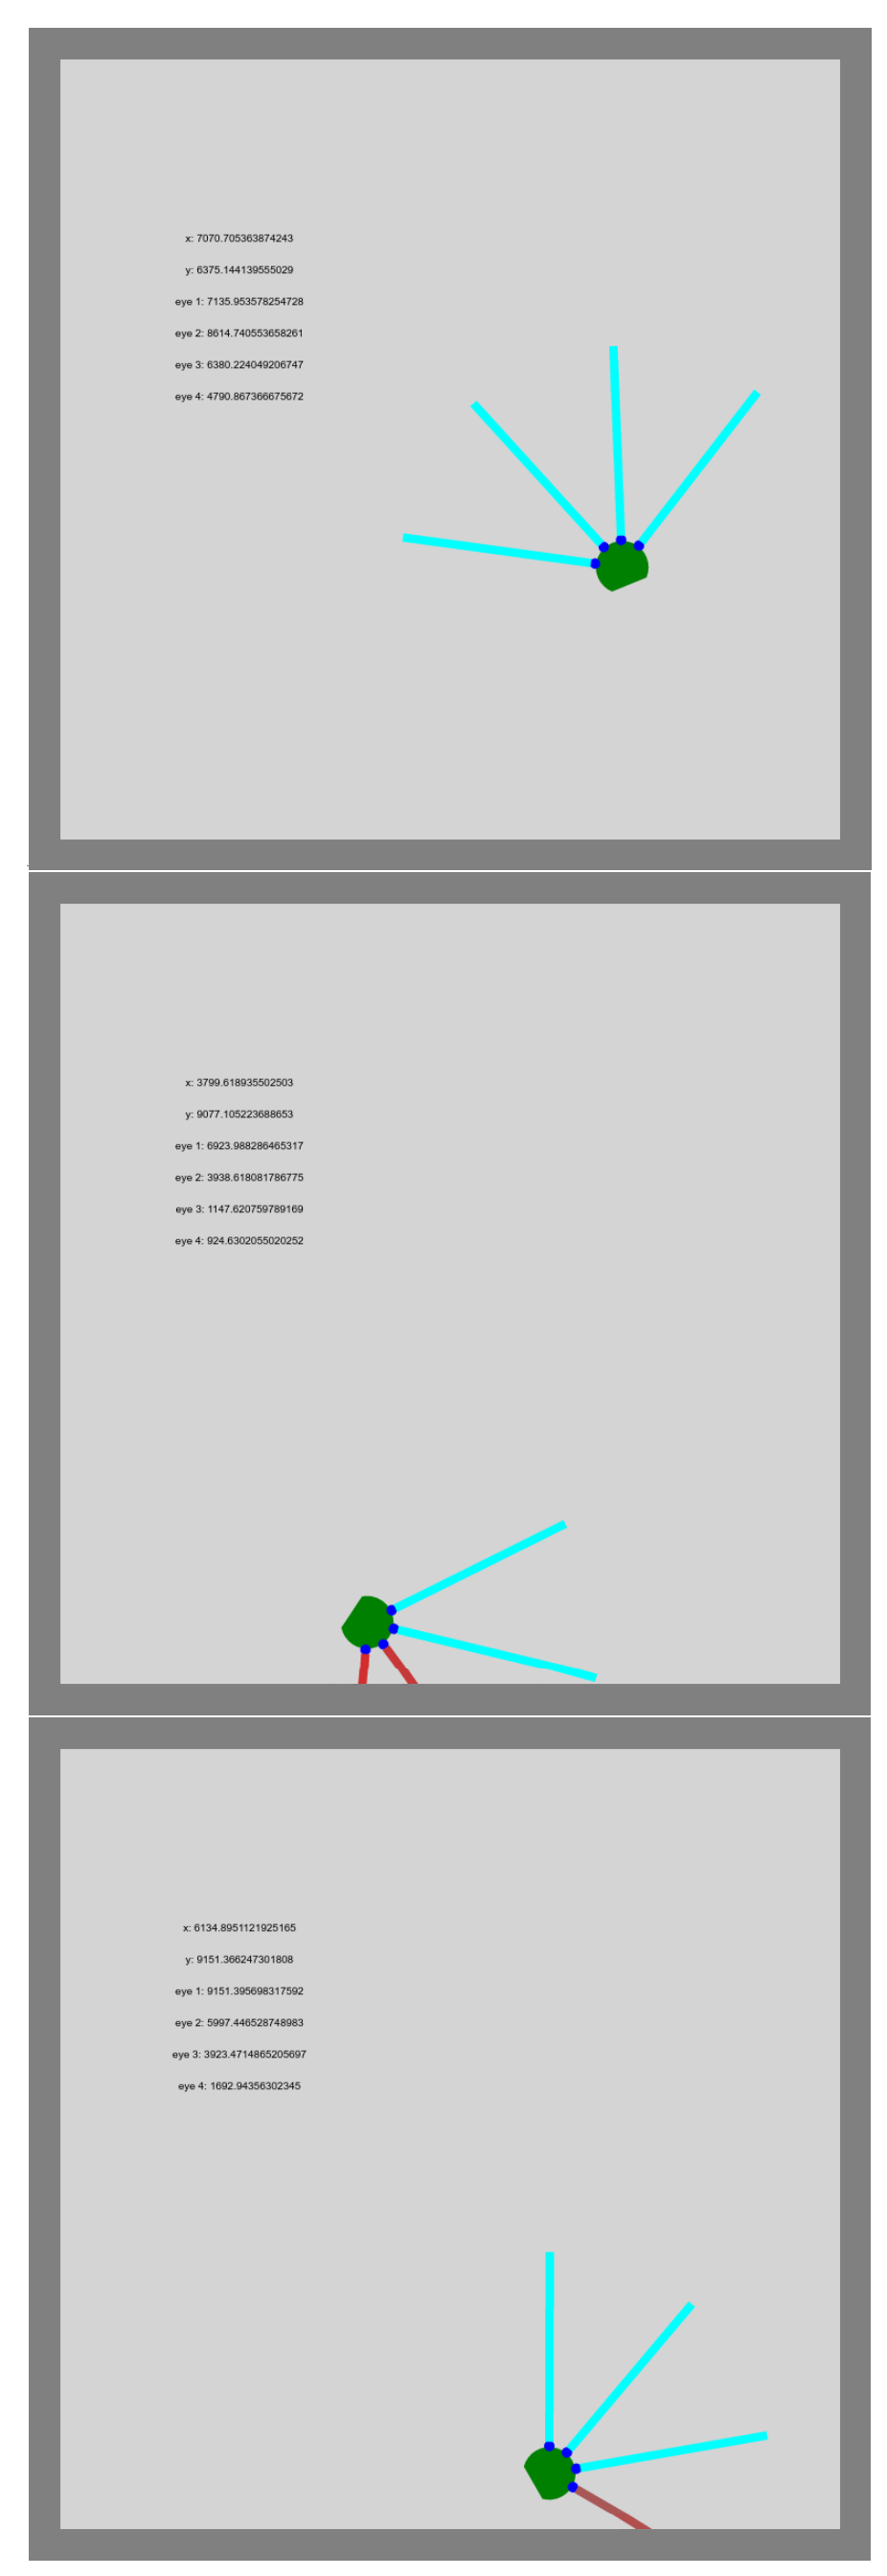
\includegraphics[width=6cm]{images/trips.png}
    \caption{A simulated agent responding to random data.\\
      In the first image the agent does not see any obstacle, \\
      while in the two lower images the agent sees the wall,\\
      visualized as the sensor indicator turning red.}
    \label{fig:screenshot}
\end{figure}
A working implementation of the system has been run, using data from an empty
micro electrode array to simulate real conditions.
The random data produced by the empty micro electrode array was received at
remote computer via TCP/IP and translated into actions for a simulated agent by
a simple untrained feed forward artificial neural network acting as a stand in
for a filter trained to interact with a neural reservoir.
\ref{fig:screenshot} shows a series of screenshots visualizing the running agent
responding to this random data.
The movement of the agent is random just like the input data, while it looks like it might be
attempting to avoid a wall this is due to chance.
In the test the sensory data perceived by the agent is sent back via TCP/IP to
the computer interfacing with the empty micro electrode array which is
stimulated.
The result of the test is that a closed loop has been successfully run, showing
that the architecture of the cyborg project is capable of handling the practical
challenges involved.
The visualizer shown in \ref{fig:screenshot} runs in real time in a web browser,
however it is not yet available on the internet.
%%% Local Variables:
%%% mode: latex
%%% TeX-master: "../main"
%%% End: